\documentclass[a4paper,fleqn]{cas-sc}

\usepackage[numbers]{natbib}
\usepackage[utf8]{inputenc}
\usepackage[T1]{fontenc}
\usepackage[polish]{babel}
\usepackage{amsmath,amssymb}
\usepackage{graphicx}
\usepackage{hyperref}

\begin{document}
\let\WriteBookmarks\relax
\def\floatpagepagefraction{1}
\def\textpagefraction{.001}

\shorttitle{Lokalne anomalie i maskowanie w algorytmie LOF -- Etap 1}
\shortauthors{J. Neugebauer, P. Moś}

\title [mode = title]{Lokalne anomalie i maskowanie odstających obiektów w LOF -- Protokół badania (Etap 1)}

\author[1]{Jakub Neugebauer}
\ead{jakub.neugebauer@student.po.edu.pl}

\author[1]{Patryk Moś}
\ead{patryk.mos@student.po.edu.pl}

\affiliation[1]{organization={Politechnika Opolska, Wydział Informatyki (Informatyka II st., Przedmiot: Rozpoznawanie wzorców, Grupa 2)},
                city={Opole},
                country={Polska}}

\begin{abstract}
Niniejszy dokument stanowi protokół badawczy dla Etapu 1 (Checkpoint 1) projektu z przedmiotu Rozpoznawanie wzorców. Celem pracy jest analiza skuteczności gęstościowego algorytmu detekcji anomalii Local Outlier Factor (LOF) w warunkach zróżnicowanej gęstości skupisk danych oraz zbadanie zjawiska wzajemnego maskowania się zgrupowanych obiektów odstających. W dokumencie zdefiniowano aparat matematyczny metody, przedstawiono ręczny przykład obliczeniowy, ustalono protokół generowania danych syntetycznych oraz zaprezentowano wstępną próbę uruchomienia modelu.
\end{abstract}

\begin{keywords}
Detekcja anomalii \sep Local Outlier Factor (LOF) \sep Gęstość lokalna \sep Zjawisko maskowania
\end{keywords}

\maketitle

\section{Wprowadzenie i przegląd literatury}
Klasyczne metody detekcji obiektów odstających (ang. \textit{outliers}) opierają się na miarach globalnych, takich jak odległość euklidesowa od globalnego centrum rozkładu. Podejście to zawodzi w przypadku zbiorów danych cechujących się obecnością klastrów o zróżnicowanej gęstości -- obiekt nieznacznie oddalony od bardzo gęstego skupiska jest intuicyjnie anomalią lokalną, mimo że jego odległość od sąsiadów jest mniejsza niż typowe odległości wewnątrz skupiska rzadkiego. Problem ten rozwiązali Breunig i in. (2000) w przełomowej pracy wprowadzającej współczynnik \textit{Local Outlier Factor} (LOF) \cite{breunig2000lof}, który zastępuje binarną decyzję o anomalii ciągłym stopniem izolacji wyznaczanym względem gęstości lokalnego otoczenia punktu.

Głównym pytaniem badawczym projektu jest ustalenie: (1) w jakich warunkach ocena lokalnej gęstości pozwala wykryć anomalie niewidoczne dla miary globalnej oraz (2) kiedy zgrupowanie anomalii w przestrzeni cech prowadzi do zjawiska maskowania ich nietypowości.

\section{Podstawy teoretyczne i przykład obliczeniowy}
Dla ustalonego parametru $k \in \mathbb{N}_+$ (liczby sąsiadów) oraz metryki odległości $d(p, o)$, algorytm LOF definiuje cztery kluczowe wielkości:
\begin{enumerate}
    \item \textbf{Odległość $k$-tego sąsiada ($k\text{-distance}(p)$):} odległość punktu $p$ od jego $k$-tego najbliższego sąsiada w zbiorze danych. Zbiór obiektów znajdujących się w odległości nie większej niż $k\text{-distance}(p)$ oznaczany jest jako $N_k(p)$ (w przypadku remisów zbiór $N_k(p)$ może zawierać więcej niż $k$ elementów).
    \item \textbf{Odległość osiągalności (ang. \textit{reachability distance}):} wygładzona miara odległości punktu $p$ względem sąsiada $o$, zdefiniowana z użyciem $k\text{-distance}$ \textbf{sąsiada $o$} (a nie ocenianego punktu $p$):
    \begin{equation}
        \text{reach-dist}_k(p, o) = \max \{ k\text{-distance}(o), d(p, o) \}
    \end{equation}
    Zastosowanie $k\text{-distance}(o)$ stabilizuje estymację dla punktów leżących bardzo blisko siebie i zabezpiecza przed problemem bardzo małych odległości (dla duplikatów o $d(p,o)=0$ wartość nie spada poniżej $k\text{-distance}(o)$, chyba że więcej niż $k$ punktów pokrywa się w jednym miejscu).
    \item \textbf{Lokalna gęstość osiągalności (ang. \textit{local reachability density}, $lrd$):} odwrotność średniej odległości osiągalności punktu $p$ od jego sąsiadów ze zbioru $N_k(p)$:
    \begin{equation}
        lrd_k(p) = \left( \frac{\sum_{o \in N_k(p)} \text{reach-dist}_k(p, o)}{|N_k(p)|} \right)^{-1}
    \end{equation}
    \item \textbf{Współczynnik LOF:} średni stosunek lokalnej gęstości osiągalności sąsiadów punktu $p$ do gęstości samego punktu $p$:
    \begin{equation}
        LOF_k(p) = \frac{\sum_{o \in N_k(p)} \frac{lrd_k(o)}{lrd_k(p)}}{|N_k(p)|} = \frac{\frac{1}{|N_k(p)|} \sum_{o \in N_k(p)} lrd_k(o)}{lrd_k(p)}
    \end{equation}
\end{enumerate}
Wartość $LOF_k(p) \approx 1$ oznacza obiekt o gęstości zbliżonej do otoczenia (punkt normalny), natomiast wartości istotnie większe od $1$ wskazują na anomalię lokalną. Należy wyraźnie odróżnić ciągły ranking anomalii zwracany przez $LOF_k(p)$ od binarnej decyzji klasyfikacyjnej, która wymaga dodatkowego narzucenia progu alarmowania.

\textbf{Przykład obliczeniowy:} Rozważmy punkt $p$ o lokalnej gęstości osiągalności $lrd_k(p) = 2$ posiadający $|N_k(p)| = 2$ sąsiadów $o_1, o_2$, z których każdy charakteryzuje się gęstością $lrd_k(o_1) = lrd_k(o_2) = 4$. Podstawiając wartości do równania (3), otrzymujemy:
\begin{equation*}
    LOF_k(p) = \frac{\frac{lrd_k(o_1) + lrd_k(o_2)}{2}}{lrd_k(p)} = \frac{\frac{4 + 4}{2}}{2} = \frac{4}{2} = 2,0
\end{equation*}
Uzyskany wynik $LOF_k(p) = 2,0 > 1$ wskazuje, że otoczenie sąsiadów jest dwukrotnie gęstsze niż otoczenie badanego punktu $p$, co kwalifikuje punkt $p$ jako potencjalną anomalię lokalną.

\section{Protokół danych, metodologia i wstępna próba uruchomienia}
W celu odtworzenia własności z Rysunku 1 publikacji bazowej zaprojektowano deterministyczny generator danych w języku Python (\texttt{scikit-learn}, ziarno główne \texttt{SEED = 42}, budżet: CPU, $N = 470 \le 500$ obiektów w $\mathbb{R}^2$):
\begin{itemize}
    \item \textbf{Skupisko gęste ($C_1$):} $250$ obiektów z rozkładu normalnego o środku $(-5, -5)$ i odchyleniu $\sigma_1 = 0,4$.
    \item \textbf{Skupisko rzadkie ($C_2$):} $200$ obiektów z rozkładu normalnego o środku $(4, 4)$ i odchyleniu $\sigma_2 = 2,2$.
    \item \textbf{Anomalie ($20$ obiektów, etykieta $y=1$):} w wariancie bazowym $5$ anomalii lokalnych umieszczonych w odległości ok. $1,8$ od środka $C_1$ oraz $15$ anomalii globalnych z rozkładu jednostajnego $U(-11, 11)^2$.
\end{itemize}

\begin{figure}[h!]
    \centering
    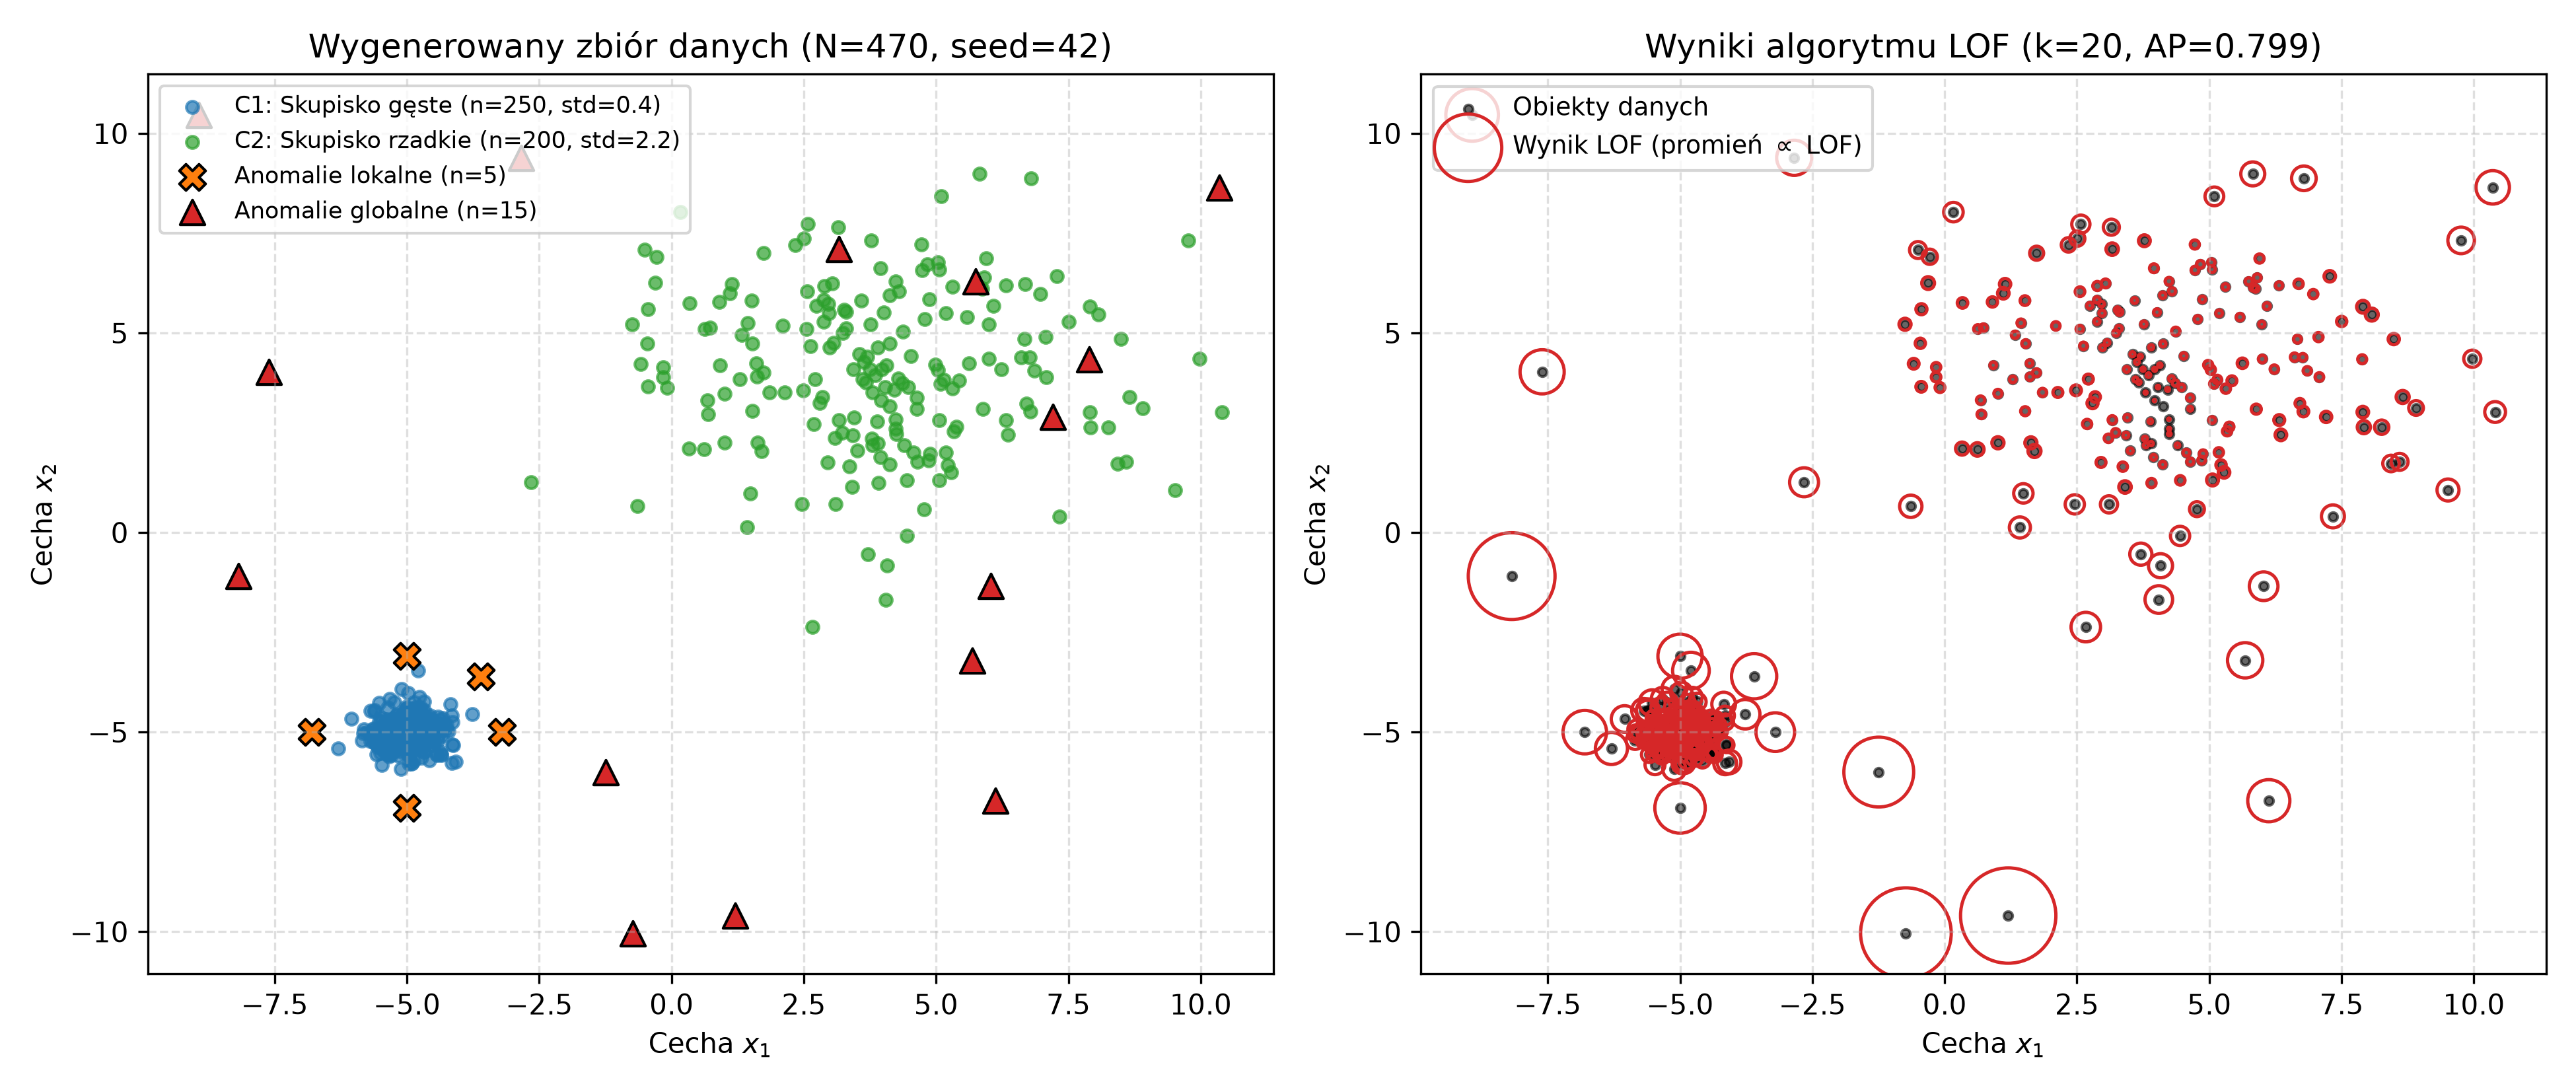
\includegraphics[width=0.92\textwidth]{stage1_dataset_preview.png}
    \caption{Wygenerowany zbiór danych syntetycznych ($N=470$) oraz wizualizacja wstępnego uruchomienia algorytmu LOF dla $k=20$.}
    \label{fig:stage1}
\end{figure}

W badaniu ustalono stałą liczbę sąsiadów $k = 20$ oraz metrykę euklidesową. Jako główną miarę oceny jakości rankingu przyjęto \textbf{Average Precision (AP)}. Istotnym elementem kontroli poprawności jest weryfikacja kierunku wyniku w bibliotece \texttt{scikit-learn}: atrybut \texttt{negative\_outlier\_factor\_} zwraca wartości ujemne ($-LOF_k$), dlatego w kodzie zastosowano odwrócenie znaku ($\text{score} = -\text{\texttt{negative\_outlier\_factor\_}}$). Wstępna próba uruchomienia (Rys. \ref{fig:stage1}) wykazała średni wynik $LOF = 1,07$ dla klastra $C_1$, $1,12$ dla klastra $C_2$, $5,97$ dla anomalii lokalnych oraz $4,82$ dla anomalii globalnych, osiągając wysoką skuteczność rankingu $\text{AP} = 0,9831$. Kod źródłowy oraz dane dostępne są w repozytorium: \url{https://github.com/columb0o/rozpoznawanie-wzorcow-lof}.

\textbf{Plan eksperymentu własnego i hipoteza dotycząca maskowania:} W kolejnych etapach, przy niezmienionych danych normalnych ($C_1, C_2$) i stałym $k=20$, dla $5$ niezależnych ziaren generatora zbadane zostaną trzy warianty rozmieszczenia $20$ anomalii: (1) pojedyncze punkty odosobnione, (2) cztery małe grupy po $5$ punktów oraz (3) jedno zwarte skupisko $20$ anomalii. Przewiduje się, że w wariancie (2) dla $k=20 > 5$ sąsiedztwo $N_k$ obejmie obiekty normalne i anomalie zostaną wykryte, natomiast w wariancie (3), gdy liczebność grupy anomalii zrówna się z parametrem $k=20$, większość sąsiadów każdej anomalii stanowić będą inne anomalie o zbliżonej gęstości $lrd$, co obniży ich współczynnik $LOF$ w okolice $1,0$ (zjawisko maskowania) i spowoduje drastyczny spadek miary Average Precision.

\section*{Podział prac i oświadczenie dotyczące wykorzystania narzędzi AI (Załącznik nr 2A)}
\textbf{Wkład autorów (Etap 1):} Jakub Neugebauer (JN) -- implementacja generatora danych syntetycznych, próba uruchomienia algorytmu LOF, wizualizacja wyników, konfiguracja repozytorium GitHub; Patryk Moś (PM) -- opracowanie aparatu matematycznego, przykład obliczeniowy, projekt protokołu eksperymentu własnego oraz redakcja tekstu.

\textbf{Wykorzystanie AI:} Przy przygotowaniu materiałów Etapu 1 wykorzystano model językowy AI (Google Gemini) w charakterze wsparcia technicznego do wygenerowania szkieletu skryptu wizualizacyjnego w bibliotece \texttt{matplotlib} oraz formatowania szablonu dokumentu w systemie \LaTeX{} (\texttt{cas-sc}). Weryfikacja wzorów matematycznych, obliczenia przykładowe, dobór parametrów protokołu oraz interpretacja wyników zostały przeprowadzone i zweryfikowane samodzielnie przez autorów.

\begin{thebibliography}{1}
\bibitem{breunig2000lof}
M. M. Breunig, H.-P. Kriegel, R. T. Ng, J. Sander, \textit{LOF: Identifying Density-Based Local Outliers}, Proceedings of the 2000 ACM SIGMOD International Conference on Management of Data, s. 93--104, 2000.
\end{thebibliography}

\end{document}